\section{Projektüberblick: Architektur}

\begin{figure}
	\centering
	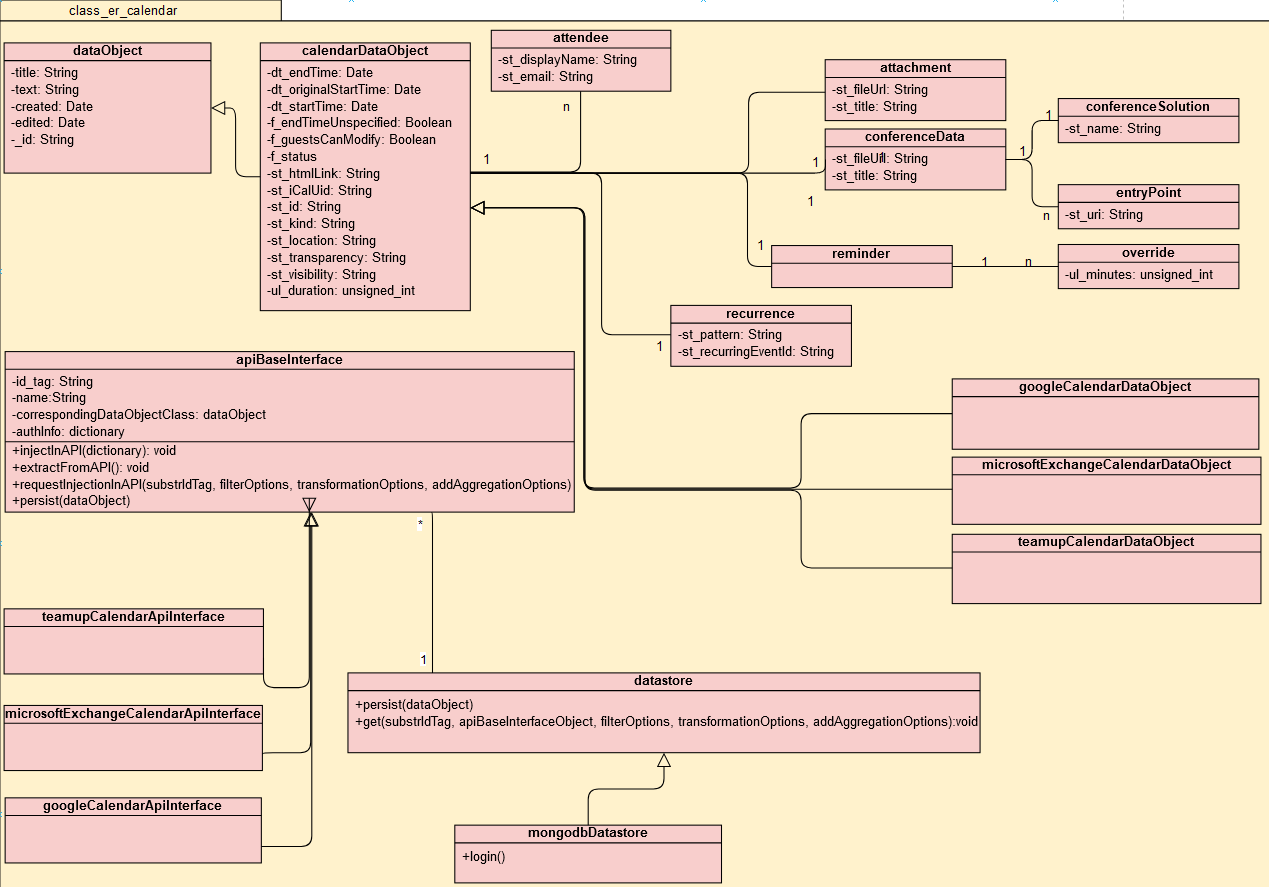
\includegraphics[width=\textwidth]{pics/architecture.png}	
	\caption{Ausschnitt aus der Architektur des Datentransformations- und Verteilungssystems}
	\label{fig:architectur}
\end{figure}

Bevor die Kalender-Services detailliert erläutert werden, ist es sinnvoll, sich einen Überblick über die Architektur des Systems zu verschaffen. Ein Ausschnitt dieser Architektur mit den wichtigsten Komponenten ist in Fig. \ref{fig:architectur} dargestellt. Für dieses Schaubild wurden aus dem Grund der Übersichtlichkeit die Attribute der konkreten Daten-Objekte die von der abstrakten Klasse calendarDataObject erben, und einige Klassen, sowie deren Attribute, die zu der Klasse calendarDataObject gehören, weggelassen.\\
Auf der obersten Ebene befinden sich die abstrakten Klassen apiBaseInterface und dataObject. Erstere definiert die benötigten Methoden um Daten aus einem Service zu lesen und zu schreiben, sowie die Schnittstelle zur konkret verwendeten Datenbank, hier die MongoDB. Bei der Abfrage der API erhält man hierbei eine komplette Liste der Ergebnisse, beim Lesen von der Datenbank wird jedoch ein Iterator für den Datensatz zurückgegeben, wodurch nicht alle Datensätze in den Arbeitsspeicher geladen werden müssen. Daher wird zwischen der Methode requestInjectionInAPI und injectInAPI unterschieden. Die Methode requestInjectionInAPI entspricht einem Aufruf der Datenbank, um alle benötigten Informationen abzufragen. Jeder somit erhaltene Datensatz wird nun innerhalb der Methode einzeln mittels der Methode injectInAPI in den konkreten Service geschrieben. Von dieser Klasse apiBaseInterface erben die konkreten Implementierungen für die verschiedenen Service-Schnittstellen, somit nutzen diese die selbe Datenbank, und müssen die immer gleichen Methoden nicht nochmals implementieren. Einzig die Methoden extractFromAPI und injectInAPI sind individuell für jeden Service und müssen überschrieben werden, sowie die Attribute des apiBaseInterface. Der id\_tag entspricht einer Zusammensetzung aus der Kategorie und dem konkreten ApiInterface-Namen, name entspricht dem Anzeigenamen in der GUI, damit die ApiInterface-Namen dem korrespondierenden Service leichter zugeordnet werden können. Zudem definiert das Attribut authInfo die benötigten Anmeldeinformationen, um sich im Service einloggen zu können, oder spezifische Daten, wie gewünschte Subkalender für die Operation angeben zu können. Um Transformationen korrekt auszuführen, muss zudem bekannt sein, welche Attribute in welchem Service existieren, hierfür kennt das konkrete ApiInterface, das zugehörige konkrete Datenobjekt. Dies würde sich auch über Konventionen für Benennungen lösen lassen, gibt dem Programmierer an dieser Stelle jedoch etwas mehr Freiheiten. \\
Die zweite abstrakte Klasse ist dataObject, diese definiert die Attribute welche über mindestens zwei Kategorien identisch sind und somit für die Transformation von Daten über Kategorien hinweg nötig sind. Die darunterliegende Hierarchie, hier calendarDataObject definiert alle Attribute, die in mehreren Kalenderservices vorhanden sind, somit befinden sich in der untersten Ebene in den konkreten DataObjects nur solche Attribute, die nur im jeweiligen Service vorzufinden sind. Eine Übersicht, welche Attribute der Kalender-Services zu den neu definierten Attribute der Datenobjekte gehören, ist unter dem Link \glqq \url{https://drive.google.com/file/d/1F3JymnclAvFreB0US2ZZT0XHX62KHEG5/view?usp=sharing}\grqq einsehbar. \\
Der Grund für die Wahl von MongoDB ist auf die Flexibilität der Speicherung zurückzuführen. Da alle Services unterschiedliche Daten zurückliefern, macht es Sinn, diese so wie sie sind, als Schlüssel-Wert-Tupel zu speichern, anstatt wie in relationalen Datenbanken üblich, eine einheitliche, hier erzeugte übergroße Struktur mit den Daten zu befüllen, wobei sehr viele Felder leer bleiben würden. \\





